\documentclass[../main.tex]{subfiles}
\begin{document}
%\chapter{Finto}
%\chapter{Finto}
%\chapter{Finto}
%\newpage
\setchapterstyle{kao}
\setchapterpreamble[u]{\margintoc}
\chapter[Differential forms I]{Differential forms I\footnotemark[0]}
\labch{diff_form_I}
\section*{Intro: two chapters}
\begin{figure}[H]
	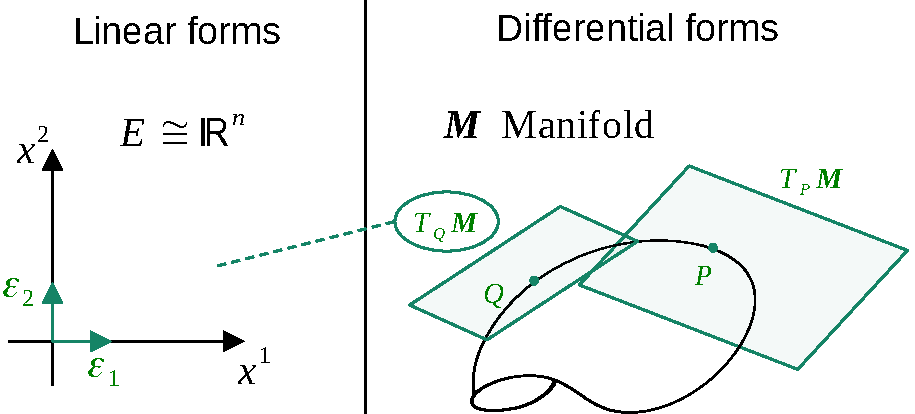
\includegraphics{images/differential_forms_scheme.pdf}
	\caption[Scheme of he chapters o differential forms]{Scheme of he chapters o differential forms}
	\labfig{diff-forms-scheme}
\end{figure}
\begin{itemize}
    \item In this chapter we speak about linear forms in the ambient of a space\sidenote{The $E$ stands for \textit{espace}, the French word for space.} $E\cong \mathbb{R}^n$ and we define some interesting objects:
    \begin{enumerate}
        \item Linear 1-form = linear functional
        \item linear 2-form = \textbf{antisymmetric} bilinear functional
        \item linear k-form = \textbf{alternating} multilinear functional
    \end{enumerate}
    This part of the theory is just multi-linear algebra.
    \item In the next chapter we speak about differential forms and the ambient is different: it is a manifold, which has the very nice property that every point is endowed with a tangent space. Since $T_Q\mathbf{M}$ is a linear space od dimension $n$, we identify it with the old one and we import all the definitions. A \textbf{differential k-form} is essentially the assignment of a \textbf{linear k-form} $\omega_P$ on every $T_P\mathbf{M}$ \textbf{for} $P\in\mathbf{M}$ that depends \textbf{"smoothly"} on $P\in \mathbf{M}$.
\end{itemize}
If we understand the first, the second ones will be easy 
\section{(Multi) linear forms}
\paragraph{\underline{Setting}: $\quad E\cong \mathbb{R}^n$}
\subsection{Linear 1-forms = linear functionals}
For completeness, let us write that
\begin{definition}[linear 1-form]
A \textbf{linear 1-form} on $E$ is a \underline{linear} 
\[
\alpha: E \to \mathbb{R}
\]
the set off all functionals is called \index{Dual space}
\[
\textrm{\textbf{Dual space}} \quad E^\ast=\left\{\alpha: E\to\mathbb{R} \ \textrm{ linear} \right\}
\]
and it is a linear space under
\[
\begin{split}
    \left(\alpha_1+\alpha_2\right)(V) &=\alpha_1(V)+\alpha_2(V)\\
    \left(\lambda\alpha\right)(V) &= \lambda\cdot\alpha(V)
\end{split}
\qquad \forall \ V\in E. \ \forall \ \lambda\in\mathbb{R}
\]
It i easy to prove that \(\textrm{dim}E^\ast=\textrm{dim}E\)
\end{definition}
\subsection{Linear 2-forms}
This is the first interesting case
\begin{definition}[linear 2-form]
a \textbf{linear 2-form} is a map
\[
\begin{split}
\eta : E\times E& \to  \mathbb{R}\\
(v,w) &\mapsto \eta(v,w)
\end{split}
\]
which is:\marginnote{
\begin{kaobox}[frametitle=Remark]
By antisymmetry \(\eta(v,v)=0 \quad \forall \ V\in E\)
\end{kaobox}
}
\begin{enumerate}
    \item bilinear;
    \item \textbf{antisymmetric} \(\quad \eta(w,v)=-\eta(v,w)\)
\end{enumerate}
\end{definition}
A very popular example which is also in \sidecite{arnold2010metodi}, is the following
\begin{marginfigure}[8mm]
	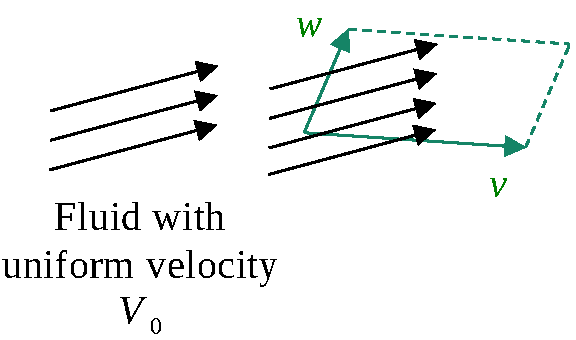
\includegraphics[width=1.1\linewidth]{images/fluid_as_linear_2form.pdf}
	\caption[Flux of a fluid as 2-form]{}
	\labfig{flux-fluid}
\end{marginfigure} 
\begin{example}
In $\mathbb{R}^3$ with the ordinary scalar product. take a fluid with uniform velocity $V_0$ in some directions. Then take two vectors which form a parallelogram. the flux of the fluid trough the surface generated by $v$ and $w$ is a \textbf{linear 2-form} that can be written as:
\[
\textrm{Flux}(v,w)=V_0\cdot(v\underset{\mathclap{\tikz \node {$\uparrow$} node [below=1ex] {\footnotesize Vector product in $\mathbb{R}^3$};}}{\times} w)
\]
it is easy to check that this is bilinear and antysymmetric.\marginnote{Anything that is constructed like that. i.e. the scalar product times a vector product is a linear 2-form.}
\end{example}
\subsection{Linear k-form}
\begin{definition}[linear k-form]
A \textbf{linear k-form}\index{Linear k-form} is a map
\[
\eta : \underbrace{E\times\dots\times E}_{\textrm{k times}} \to  \mathbb{R}\\
\]
which is
\begin{enumerate}
    \item multi-linear;
    \item \textbf{alternating}:\marginnote{This should remind us the Fermionic wave function.}
    \[
    \omega\left(v_1\dots,{\color{red}v_j},\dots,{\color{red}v_l},\dots,v_n\right)={\color{red}(-1)}\omega\left(v_1.\dots,{\color{red}v_l},\dots,{\color{red}v_j},\dots,v_n\right)
    \]
    equivalently we can write it with permutation.
\end{enumerate}
\end{definition}
The most famous multi-linear alternating form is the determinant.
\begin{example}
If $k=n$, an example is the \textbf{determinant}\index{Determinant} of $n$ vectors
\[
\begin{split}
\textrm{det} : E\times\dots\times & \to  \mathbb{R}\\
(v_1,\dots,v_n) &\mapsto \textrm{det}(v_1,\dots,v_n)
\end{split}
\]
Let us take for example the canonical bases, each one of these vectors will have components in the bases that forms a column\marginnote{The first subscript is the number of the vector and the second one identify the component.}
\[
\textrm{det}
\begin{pmatrix}
v_{1,1} & v_{2,1} & \dots & v_{n,1}\\
\vdots & \vdots & & \vdots\\
v_{1,n} & v_{2,n} & & v_{n,n}
\end{pmatrix}
\]
We discover that this number does not depend on the choice of the bases. This is multilinear (linear in each variable), alternating and eventually one can prove that is the unique n-linear form which has the value one over the canonical bases (Capitolo 9 of \sidecite{abate2006geometria}).
\end{example}
Another example is the k-volume generated by some k-vectors in the space
\begin{example}
from $2\leq k \leq n$, the volume generated by $v_1, v_2,\dots, v_k$  is a \textbf{linear k-form.}
% FINE LEZIONE 5 - 17/03/2022
% INIZIO LEZIONE 6 - 18/03/2022
%1:37:00
[Da aggiungere il grafico] Suppose we are in $\mathbb{R}^n$, with $n$ very large, we consider a \href{https://it.wikipedia.org/wiki/Parallelepipedo}{parallelepiped} generated by $(V_1,V_2,V_3)$:
\[
P(V_1,V_2,V_3)=\left\{\sum_{j=1}^3 \lambda_j V_j : 0 \le \lambda_j \le 1\right\}
\]
The \textbf{oriented} volume of $P(V_1,V_2,V_3)$ is a \textbf{linear 3-form}. The exchange of two vectors is a change of orientation in the corresponding plane, hence it results in a change of sign.
\end{example}
\begin{proposition}[Linear structure]\index{Linear structure}
The space $\Lambda^k E$ of all the linear k-forms on $E$ is a \textbf{linear space}, with the obvious definitions of linear operations:
\begin{enumerate}
\item $(\omega_1+\omega_2)(V_1,\dots,V_k)=\omega_1(V_1,\dots,V_k)+\omega_2(V_1,\dots,V_k)$
\item $(\lambda\omega)(V_1,\dots,V_k)=\lambda\cdot\omega(V_1,\dots,V_k)$
\end{enumerate}
$\forall\lambda\in\mathbb{R},\forall\omega,\omega_1,\omega_2\in\Lambda^kE$
\end{proposition}
\begin{proof}
Exercise. \sidecite{doCarmo1994}
\end{proof}
\section{The wedge product of forms}\marginnote{"\href{prodotto esterno}{Prodotto esterno}" in italian.}
If we have a k-form $\omega$ and a p-form $\eta$, then the wedge product $\omega\wedge\eta$ \textbf{is a (k+p)-form}. To define it, pedagogically is better to distinguish the cases.
\subsection{\underline{Case I}}Let us now consider two 1-forms $\alpha_1$ and $\alpha_2$:
\begin{definition}[Wedge product of 1-forms]\index{Wedge product of 1-forms}
The \textbf{wedge product} $\alpha_1\wedge\alpha_2\in\Lambda^2 E$ is defined as:
\begin{align*}
(\alpha_1\wedge\alpha_2)(V_1,V_2)
&=\alpha_1(V_1)\alpha_2(V_2)-\alpha_2(V_1)\alpha_1(V_2)=\\
&=\textrm{det}\begin{pmatrix}
\alpha_1(V_1) & \alpha_1(V_2)\\
\alpha_2(V_1) & \alpha_2(V_2) 
\end{pmatrix}
\end{align*}
\end{definition}
\begin{marginfigure}[8mm]
	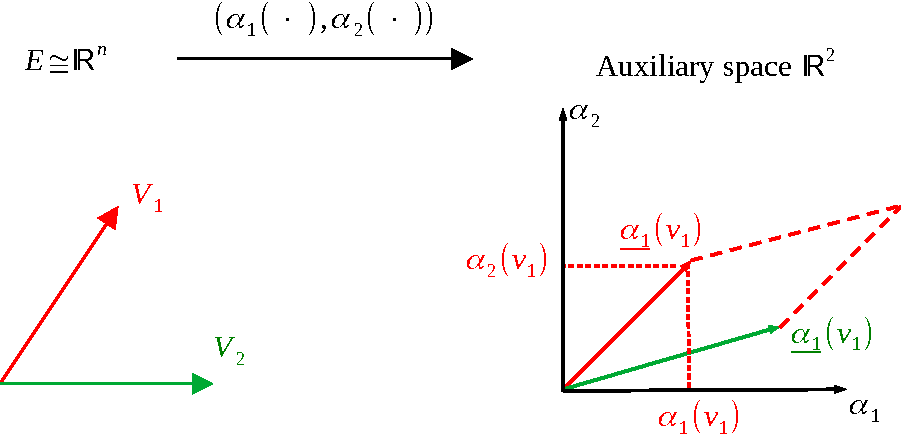
\includegraphics[width=1.1\linewidth]{images/geom_explanation.pdf}
	\caption{Scheme of the geometric explanation.}
	\labfig{geom-expl}
\end{marginfigure}
\begin{kaobox}[frametitle=Remark: Geometric meaning]
Let us take $E\cong\mathbb{R}^n$. Imagine to have a map which goes to the physical space (in the sense of our reference space) to the non-trivial space obtained by:
\[
E\ni V \mapsto (\alpha_1(v),\alpha_2(v))\equiv\underline{\alpha}(v)\in\mathbb{R}^2
\]
Which means that with the help of the two 1-forms, we have a description in an auxiliary space. More precisely, the number $(\alpha_1\wedge\alpha_2)(v_1,v_2)$ is the \textbf{oriented area} of the parallelogram generated by $\underline{\alpha}(v_1)$ and $\underline{\alpha}(v_2)$ in the auxiliary space $\mathbb{R}^2$.
\end{kaobox}
\marginnote{Sometimes we will say "volume", but a volume in the dimension two is an area.}

\begin{example}
Prove that $(\alpha_1\wedge\alpha_2)$ is indeed a linear 2-form.
\end{example}
\begin{example}
Prove that:
\begin{enumerate}
    \item $(\alpha\wedge\eta)=-(\eta\wedge\alpha)$
    \item $(\lambda_1\alpha_1+\lambda_2\alpha_2)\wedge\eta=\lambda_1\alpha_1\wedge\eta+\lambda_2\alpha_2\wedge\eta$ \\
    $\text{for all } \lambda_1,\lambda_2\in\mathbb{R} \text{ ; } \alpha,\eta,\alpha_1,\alpha_2\in\Lambda^1 E$
\end{enumerate}
\end{example}
We can \textbf{iterate the wedge product}. If $\alpha_1,\alpha_2,\dots,\alpha_k$ are \textbf{linear 1-forms} we get
\[
(\alpha_1\wedge\dots\wedge\alpha_k)(V_1,\dots,V_k)=\det\begin{pmatrix}
\alpha_1(V_1) & \cdots & \alpha_1(V_k)\\
\vdots & \ddots & \vdots \\
\alpha_k(V_1) & \cdots & \alpha_k(V_k)
\end{pmatrix}
\]
The geometric interpretation is similar to the case where $\boxed{k=2}$, i.e. the \textbf{oriented volume} of a \textbf{k-}parallelepiped in an auxiliary space $\mathbb{R}^k$.
\paragraph{+ The "monomials" for the wedge products}
So far, everything was \textbf{coordinate-free}. Now we consider a linear basis $\{e_1,\dots,e_n\}$ for $E$ so that $V=\sum_{j=1}^{n}v^j e_j$. We take into account the \textbf{dual basis} $\{dx^1,\dots,dx^n\}$ defined as

\begin{marginfigure}[8mm]
	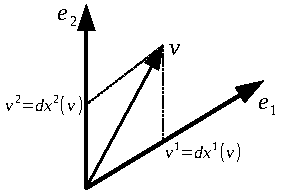
\includegraphics[width=1.1\linewidth]{images/dual_basis.pdf}
	\caption{Scheme of the representation of $v$ in the dual basis.}
	\labfig{dual-basis}
\end{marginfigure}

\[
dx^j(V)=v^j
\]
$dx^j:E\to\mathbb{R}$ linear, is a \textbf{linear functional}, i.e. a \textbf{linear 1-form} so we can consider the wedge-product:
\[
\begin{split}
dx^j\wedge dx^l(V,W)=v^j w^l-v^l w^j &\text{ is a linear 2-form} \ \left(j,l\in\left\{1,\dots,n\right\}\right)\\
dx^j\wedge dx^l\wedge dx^m \qquad\qquad\qquad \ \ &\text{ is a linear 3-form}
\end{split}
\]
We can "build" k-forms simply by linear combination of this"monomials":
\begin{itemize}
    \item 1-forms $\alpha=\sum_{j=1}^n A_j dx^j$
    \item 2-forms $\beta=\sum_{j,l=1}^n dx^j\wedge dx^l$
\end{itemize}
{\fontencoding{U}\fontfamily{futs}\selectfont\char 66\relax} But \textbf{not} all the "monomials" are \textbf{linearly independent} (for $k\ge2$): $(dx^1\wedge dx^2)=-(dx^2\wedge dx^1)$ are linearly dependent. What is a maximal set of linearly independent monomials? The one which has the indices only in increasing order:
\begin{itemize}
    \item $\{dx^1\wedge dx^2\}$
    \item $\{dx^1\wedge dx^2, dx^1\wedge dx^3, dx^2\wedge dx^3\}$, the "brothers" are obtaines by permutations
\end{itemize}

\begin{proposition}
Let $E\cong\mathbb{R}^n$. Then for any $k\le n$ the \textbf{k-forms} given by the monomials $\{dx^{i_1}\wedge\dots\wedge dx^{i_n}\}$, with the fundamental \textbf{constraint} that\\
$i_1<i_2<\dots<i_n$, are \textbf{linearly independent} and generate $\Lambda^k E$ (i.e. they are a linear basis for $\Lambda^k E$).
\end{proposition}
\begin{proof}
The proof can be found in Chapter 1 of \sidecite{doCarmo1994}.
\end{proof}
\begin{corollary}
Let us consider a space $E$ with dimension $\textrm{dim}E=n$. We are interested in the dimension of $\Lambda^k E$.
For a general value of $k$: \[\textrm{dim}\Lambda^k E=\binom{n}{k}\]
\end{corollary}
For example,\marginnote{with \# we denote the number of groups $(i_1,\dots,i_n)$ which satisfy the stated condition.}
    \[
    \begin{split}
    \boxed{k=1}\quad &\Lambda^1 E=E^\ast\ , \ \textrm{the dimension is }n\\
    \boxed{k=2}\quad &\textrm{dim}\Lambda^2 E=\texttt{\#}\{(i_1,i_2):i_1<i_2\}=\binom{n}{2}=\frac{n(n-1)}{2}\\
    \boxed{k=3}\quad &\textrm{dim}\Lambda^3 E=\texttt{\#}\{(i_1,i_2,i_3):i_1<i_2<i_3\}=\binom{n}{3}
    \end{split}
    \]
\begin{kaobox}[frametitle=Remark: the miracle of $\mathbb{R}^3$]
Let us suppose to have $E\cong\mathbb{R}^3$, we have that $\textrm{dim}E=\textrm{dim}E^*=3$. If we look at $\Lambda^2 E$ we see that dim$\Lambda^2 E=\binom{3}{2}=\frac{3!}{2!(3-2)!}=3$.
Vectors (1-forms), and 2-forms have the same dimension
\[
\textrm{vectors} \ \longleftrightarrow \textrm{linear 2-forms}
\]
So for example:\textrm{Nota: the matrix is antisymmetric.}
\[
\vec{B}=\begin{pmatrix}
B_x\\B_y\\B_z
\end{pmatrix}\longleftrightarrow\begin{pmatrix}
0 & B_z & -B_y\\
-B_z & 0 & B_x\\
B_y & -B_x & 0
\end{pmatrix}=\mathbb{B}
\]
The identification is that instead of looking at $\vec{B}$, we will consider the 2-form:
\[
\beta=\sum_{i,j} \mathbb{B}_{ij}dx^i\wedge dx^j\underset{\mathclap{\tikz \node {$\uparrow$} node [below=1ex] {\footnotesize $\beta$ is an \underline{intrinsic} object};}}{=}\sum_{i,j} \Tilde{\mathbb{B}}_{ij}d\Tilde{x}^i\wedge\Tilde{x}^j
\]
where the number of contravariant indices is equal to the number of covariant indices.\marginnote[-15mm]{It is not by chance that we used the letter $\mathbb{B}$, because this is exactly the natural description of the magnetic field. In the XIX century people described it has vector field, but then people realised that the right language of the electromagnetic field was the language of differential forms.}
\end{kaobox}
\begin{corollary}
Every k-form $\omega\in\Lambda^k E$ is decomposed \textbf{uniquely} on the basis of \textbf{independent monomials}:
\[
\omega=\sum_{\color{red}i_1<\dots<i_k}\omega_{i_1<\dots<i_k}dx^1\wedge\dots\wedge dx^k
\]
\end{corollary}
\underline{E.g.} every $\beta\in\Lambda^2 E$ is written uniquely as $\beta=\sum_{\color{red}i<j}\beta_{ij}dx^i\wedge dx^j$. If $n=2$, every $\beta\in\Lambda\mathbb{R}^2$ is $\beta=bdx^1\wedge dx^2$.
\subsection{\underline{Case II:} General wedge product}Let us now consider a k-form $\omega$ and a p-form $\eta$: the wedge product $\omega\wedge\eta=??$ should be a (k+p)-form. The only natual definition is the following
\begin{definition}[General wedge product]\index{General wedge product}
The general wedge product of $\omega$ and $\eta$ is
\[
(\omega\wedge\eta)(V_1,\dots,V_{k+p})= \underset{\mathclap{\tikz \node {$\uparrow$} node [below=1ex] {\footnotesize Sum on all the possible choices };}} \sum(-1)^{\nu}\omega \overbrace{(V_{i_1},\dots,V_{i_k})}^{\textrm{choice of k vectors}} \eta \underbrace{(V_{j_1},\dots,V_{j_p})}_{\textrm{choice of p vectors}}
\]
where a "choice" $(i_1,\dots,i_k,j_1,\dots,j_p)$ is a \textbf{permutation} $\nu$ of $(1,\dots,k,k+1,\dots,k+p)$ and $(-1)^{\nu}$ is the \textbf{parity of the permutation} $\eta$.
\end{definition}
And just for information (we will not use it very often), the following proposition is true
\begin{proposition}
The general wedge product has the following properties:
\begin{enumerate}
    \item \textbf{pseudo-}commutative: $\omega\wedge\eta=(-1)^{k\cdot p}(\eta\wedge\omega)$, where $k=\deg\omega$ and $p=\deg p$
    \item distributive: $(\lambda_1\omega_1+\lambda_2\omega_2)\wedge\eta=\lambda_1(\omega_1\wedge\eta)+\lambda_2(\omega_2\wedge\eta)$
    \item associative: $(\omega\wedge\eta)\wedge\beta=\omega\wedge(\eta\wedge\beta)$
\end{enumerate}
\end{proposition}
\end{document}